\section{Ejercicio 8}

En el ejercicio 8 se pide realizar una implementación del scheduler round robin, pero sin migración de procesos entre núcleos.
Para esto se agregaron nuevas estructuras a la clase SchedRR2:
\begin{itemize}
\item \textbf{colaReady}: Ahora es un vector de colas, las cuales van a almacenar los pid de las tareas que ultilicen el core correspondiente.
\item \textbf{cantTasks}: Indica la cantidad de tareas que tiene cada cpu (RUNNING + BLOCKED + READY).
\item \textbf{cpuTareasBloqueadas}: Es una cola de tuplas con un pid en la primera coordenada (proceso que hizo llamada bloqueante) y número de core en el cual estaba ejecutando.
\end{itemize}

Los métodos load, unblock y tick también cambian respecto del round robin con migración de procesos.

\begin{itemize}
\item \textbf{load(pid)}: Se encarga primero de buscar cual es el cpu con menor cantidad de tareas y, una vez encontrado, sumar uno a la cantTasks de ese cpu. Luego encola la tarea en la cola correspondiente de tareas ready.
\item \textbf{unblock(pid)}: Como se pide que no haya migración de procesos entre núcleos, se guarda en la estructura $cpuTareasBloqueadas$ todos las tareas bloqueadas con su número de core. Esta función encuentra la tupla en la cola, la quita de la cola, y luego encola la tarea en la colaReady del cpu obtenido.
\item tick(cpu, m): Motivo TICK sigue siendo similar a la implementación anterior. Motivo BLOCK ademas de quitar al pid de la $colaReady$ del cpu, arma una tupla de la forma (pid, cpu), siendo pid = current_pid(cpu). Luego encola esa tupla en $cpuTareasBloqueadas$, si quedan tareas en la $colaReady$ toma la primera y devuelve su pid, y sino hay mas ready, devuelve IDLE_TASK. Motivo EXIT acá se resta uno a la cantTasks del cpu actual, y se devuelve la tarea que sigue en la $colaReady$ y si no hay mas, IDLE_TASK.
\end{itemize}


Para corroborar su correcto funcionamiento se ideó un lote de tareas que permita chequear que, efectivamente no haya migración de núcleos y que se asignen correctamente 
los cores que cada tarea va a utilizar. 

Lote utilizado:\\

\noindent TaskCPU 20		\\
TaskConsola 20 1 5	\\
TaskCPU 5\\
@2: \\
*2 TaskCPU 20\\
TaskCPU 5\\
@4:\\
TaskCPU 20\\
TaskConsola 10 1 5\\
TaskConsola 2 1 2\\
@18:	\\			
TaskCPU 5\\
TaskConsola 3 2 4\\

La simulación se hizo con 3 cores con cambio de contexto 0, ya que no modifica el comportamiento del scheduler, y el costo de migración de núcleo 0.
La idea del lote, es cargar los primeros cores con tareas que tarden más en terminar, y dejar en el último tareas que vayan terminando y que liberen el cpu, para poder apreciar de esta forma, que efectivamente se asignará el cpu con menos tareas.
Debido a la implementación, cuando todos los cores tengan igual cantidad de procesos, se le asignará el cpu más chico numéricamente. 

\newpage

\begin{figure}[h]
  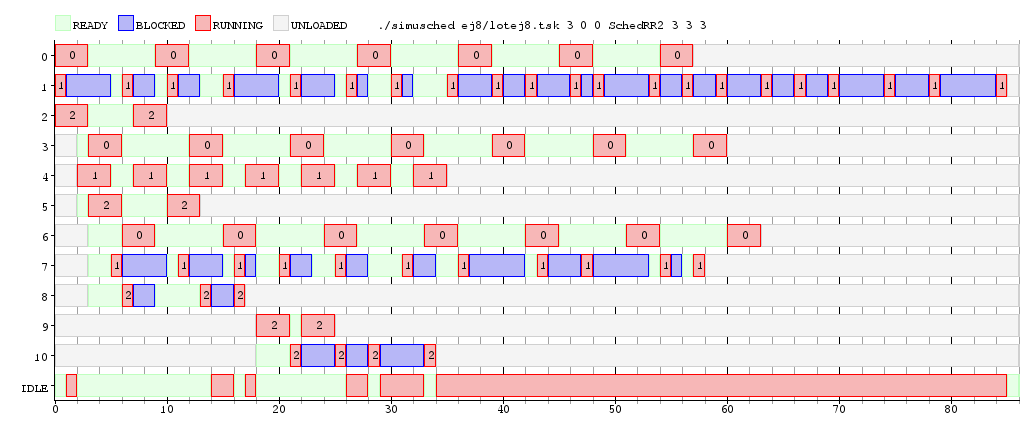
\includegraphics[width=\textwidth]{../ej8/rr2.png}
  \caption{}
\end{figure}

Se puede observar que no existe migración de núcleos, ya que todas las tareas mantienen su número de cpu a lo largo de toda la simulación.
En los instantes 0, 2 y 4 llegan las tareas y se les asignan los cores de la forma esperada. En el instante 4, los 3 cpu tienen 3 tareas cada uno.
En el instante 15 el cpu 2 se queda sin tareas para ejecutar(la tarea 2 termina en el momento 2, la 5 en el 9 y la 13 en el 15). 
Por lo tanto se le asigna el IDLE_TASK por un ciclo de clock hasta que llegan dos nuevas tareas. Vemos que efectivamente se le asignan al core número 2,
que es el que menos tareas tenía de los tres. En el tick 32, la tarea 10 hace EXIT y el cpu 2 no tiene mas tareas que ejecutar.
Este representa una gran desventaja, ya que mientras los dos primeros cpu están trabajando y tienen tareas esperando, el cpu 2 permanece inactivo.
Esto pasa porque el único método de equilibrado de carga que se implementa es comprobar que cpu tiene menos tareas. Para mejorar el uso de cpu o equilibrar la cantidad de 
trabajo de cada core, se podría implementar la $migración\ solicitada$, que hace que se pasen tareas a un cpu que esté inactivo (sin tareas bloqueadas).\\


Por otro lado, matener un proceso siempre en un mismo núcleo tiene sus ventajas. Por ejemplo, si se considera lo que ocurre con la memoria
caché cuando una tarea se estuvo ejecutando en un cpu específico: los datos a los que el proceso ha accedido mas recientemente se almacenan en la caché de ese
procesador, luego gran parte de accesos a memoria se evitan ya que los datos se encuentran en la caché. Además si se produjera una migración de núcleo, los datos de
esa caché deberían invalidarse, y luego debería llenarse la caché del nuevo cpu. 
Este concepto se lo llama $afinidad\ al\ procesador$, que es que cada proceso tiene una afinidad al cpu en el que esta ejecutando. En esta implemetación, se 
utiliza $afinidad\ dura$, que no permite la migración entre cores. También existe la $afinidad\ suave$, en este caso es posible que una tarea cambie de cpu. \\

Para ver el beneficio de la $afinidad\ dura$ se construyó el siguiente lote de tareas: \\

\item *4 TaskCPU 100

\\
\newpage
Se realizó una simulación con la primera implementación de Round Robin, que permitía la migración, y una con la que no.
Para tener en cuenta los costos de tiempo de invalidar la caché y rellenarla cada vez que se cambie de núcleo, se estableció 4 ticks como costo de migración de cpu.
Hay que tener en cuenta que el simulador no provee funciones que permitan emular el uso de la memoria caché, es decir, no se va a poder medir cantidad de accesos
a memoria y accesos a chaché.
La simulación se realizó con 3 cores, y todos con misma cantidad de quantum.




\begin{figure}[h]
  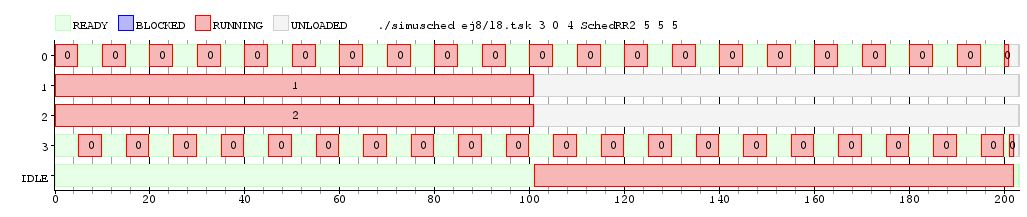
\includegraphics[width=\textwidth]{../ej8/rr24task.png}
  \caption{Round Robin Sin migración.}
\end{figure}

\begin{figure}[h]
  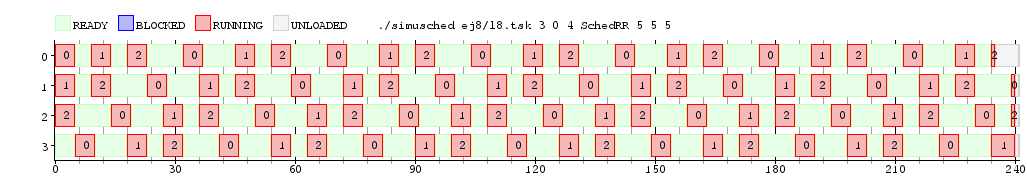
\includegraphics[width=\textwidth]{../ej8/rr4task.png}
  \caption{Round Robin Con migración.}
\end{figure}


A simple vista, se ve como el $tiempo\ de\ ejecución$ mejoró respecto de la primera implementación de Round Robin. En el gráfico 15 
se ve que recién en el instante 234 termina la primera tarea del lote y en el 240 las últimas 2. En el gráfico 14 vemos que las dos útlimas tareas
terminan en el tick 205 aproximadamente. 
Notar también como a partir del instante 100 del gráfico 14, tanto el cpu 1 como el 2 quedan inactivos por mas de 100 ciclos. Esta desventaja se describió en el 
primer ejemplo.



